\documentclass{article}
\usepackage{graphicx}
\usepackage{amsmath}
\usepackage{acronym}
\usepackage[backend=bibtex]{biblatex}

\title{Aposteriori Unimodality}
\author{Dimitris Tsirmpas, John Pavlopoulos}
\date{March 2025}


% Insert space after commas in math mode
\AtBeginDocument{%
  \mathchardef\stdcomma=\mathcode`,
  \mathcode`,="8000
}
\begingroup\lccode`~=`, \lowercase{\endgroup\def~}{\stdcomma\,}

\graphicspath{ {../graphs} {graphs}  }
\bibliography{refs.bib}


\begin{document}

\maketitle

\section{Methodology}

In this section, we provide a formal mathematical formulation of the problem of attributing polarization to specific annotator characteristics (\S\ref{ssec:methodology:problem}), and offer an intuitive rationale for how established polarization metrics can be leveraged in this context (\S\ref{ssec:methodology:intuition}). We then introduce a data-point-level measure that attributes polarization to individual \ac{SDB} factors (\S\ref{ssec:methodology:polstat}), and subsequently develop a statistical test that formalizes this attribution in a robust manner. Finally, we outline the technical details of the proposed methodology (\S\ref{ssec:methodology:details}).

\subsection{Problem Formulation}
\label{ssec:methodology:problem}

Let $d = \{c_1, c_2, \ldots\}$ be a dataset $d$ composed of $\lvert d \rvert$ annotated data-point. We assume that annotating a data-point depends on three variables: its contents, the annotator's \ac{SDB}, and uncontrolled factors such as mood and personal experiences. Assuming that each data-point $c$ is assigned multiple annotators, we can define the annotation set $A(c)$ as:
\begin{equation}
    A(c) = \{a(c; \theta) \mid \theta \in \Theta \}
\end{equation}
\noindent where  $a(c; \theta)$ is a single annotation for data-point $c$ and $\Theta$ is the set of annotator \acp{SDB}.

Each set of annotations features a certain degree of \textit{polarization}. Unpolarized annotations are usually unimodal, which makes intuitive sense. Even in scenarios with high inter-annotator disagreement, there is a difference between the annotators disagreeing on the details (which would be shown roughly as a bell curve around the median annotation), and them fundamentally disagreeing with each other (which would likely be shown as a multimodal distribution). \textcite{pavlopoulos-likas-2024} create a polarization metric, the ``\ac{nDFU}'', which measures whether an annotation set shows no polarization (unimodal distribution --- $nDFU=0$), up to complete polarization (multimodal distribution --- $nDFU=1$). 

Since our goal is to pinpoint which specific characteristics contribute to polarization, we need to isolate individual groups within a \ac{SDB}. $\Theta$ can be one of multiple ``dimensions'' (e.g., age, sex, educational level), which are composed of various groups ($\theta_1, \theta_2, \ldots \in \Theta$). Thus, we will define a test that, given that annotation polarization exists, tests whether the \ac{nDFU} of a data-point's annotations can be partially explained by $\theta_i$.


\subsection{Quantifying changes in polarization}
\label{ssec:methodology:intuition}

Intuitively, $\theta_i$ partially explains the polarization of a data-point $c$ when the annotations made by annotators with $\theta_i$ are more polarized compared to the full set of annotations. Figure~\ref{fig:ndfu_single_data-point} exhibits a hypothetical example where a misogynistic comment is annotated for toxicity by male and female annotators. The annotations are generally polarized ($nDFU_{all} = 0.625$), although the set of annotations from female annotators might exhibit low polarization between themselves ($nDFU_{women} = 0.1$---most agree the data-point is toxic). The set of male annotations on the other hand, also shows low polarization ($nDFU_{men} = 0.3725$), but for the opposite reason---most men agree that it is \emph{not} toxic. This suggests that the overall polarization is driven by disagreements between male and female annotators.

\begin{figure}
	\centering
	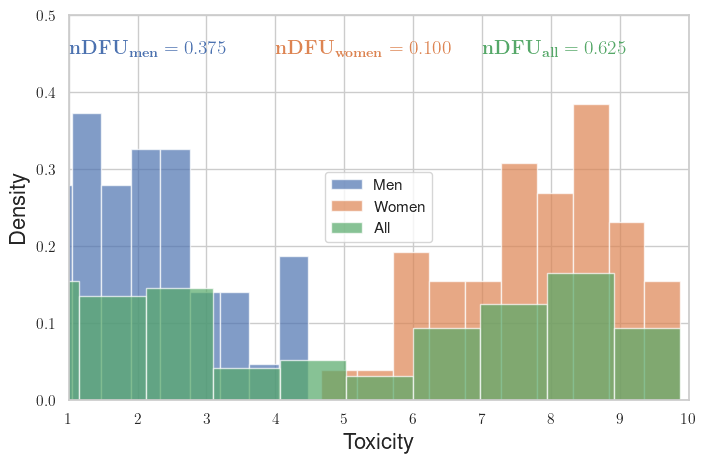
\includegraphics[width=0.8\linewidth]{ndfu_combined.png}
	\caption{Hypothetical example of a polarizing data-point, where male and female annotators agree between themselves, but disagree with the opposite gender. Overall polarization ($nDFU_{all} = 0.625$) is much greater than the polarization exhibited by the annotations grouped by gender ($nDFU_{men} = 0.3725, nDFU_{women} = 0.1$). %In this example, the annotation set $A$ was generated as $A_{men} \sim \mathcal{N}(2, 1.3), A_{women} \sim \mathcal{N}(8, 1.3), \lvert A_{men} \rvert = \lvert A_{women} \rvert = 50$.
    }
	\label{fig:ndfu_single_data-point}
\end{figure}

Given this observation, we would be tempted to aggregate all annotations in the dataset and compare the polarization of each $\theta_i$ with that of $\Theta$. However, this formulation would not work well. Figure~\ref{fig:ndfu_multi_data-point} illustrates a hypothetical discussion with two comments, both of which are toxic, but where male and female annotators disagree on \emph{which} comment is the toxic one. If we aggregate the annotations to a single discussion, the opposing polarization effects might balance each other out, leading to a false negative. In simpler terms, polarization has a \textit{direction}, and care must be taken to not combine polarization effects of opposite directions.

In our example, while it is obvious that gender partly explains the polarization found in each of the individual comments ($nDFU_{all} \gg nDFU_{men}, nDFU_{all} \gg nDFU_{women}$), this observation is much harder to make when aggregating the two comments. This is graphically shown as the presence of three bimodal distributions instead of two unimodal distributions, and one bimodal (aggregated) distribution. To avoid this, we apply our statistic only on annotations that reference the same data-point.

\begin{figure*}
	\centering
    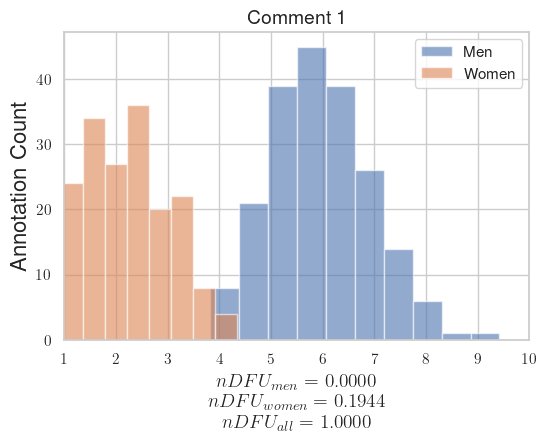
\includegraphics[width=0.3\linewidth]{ndfu_comment1.png}
    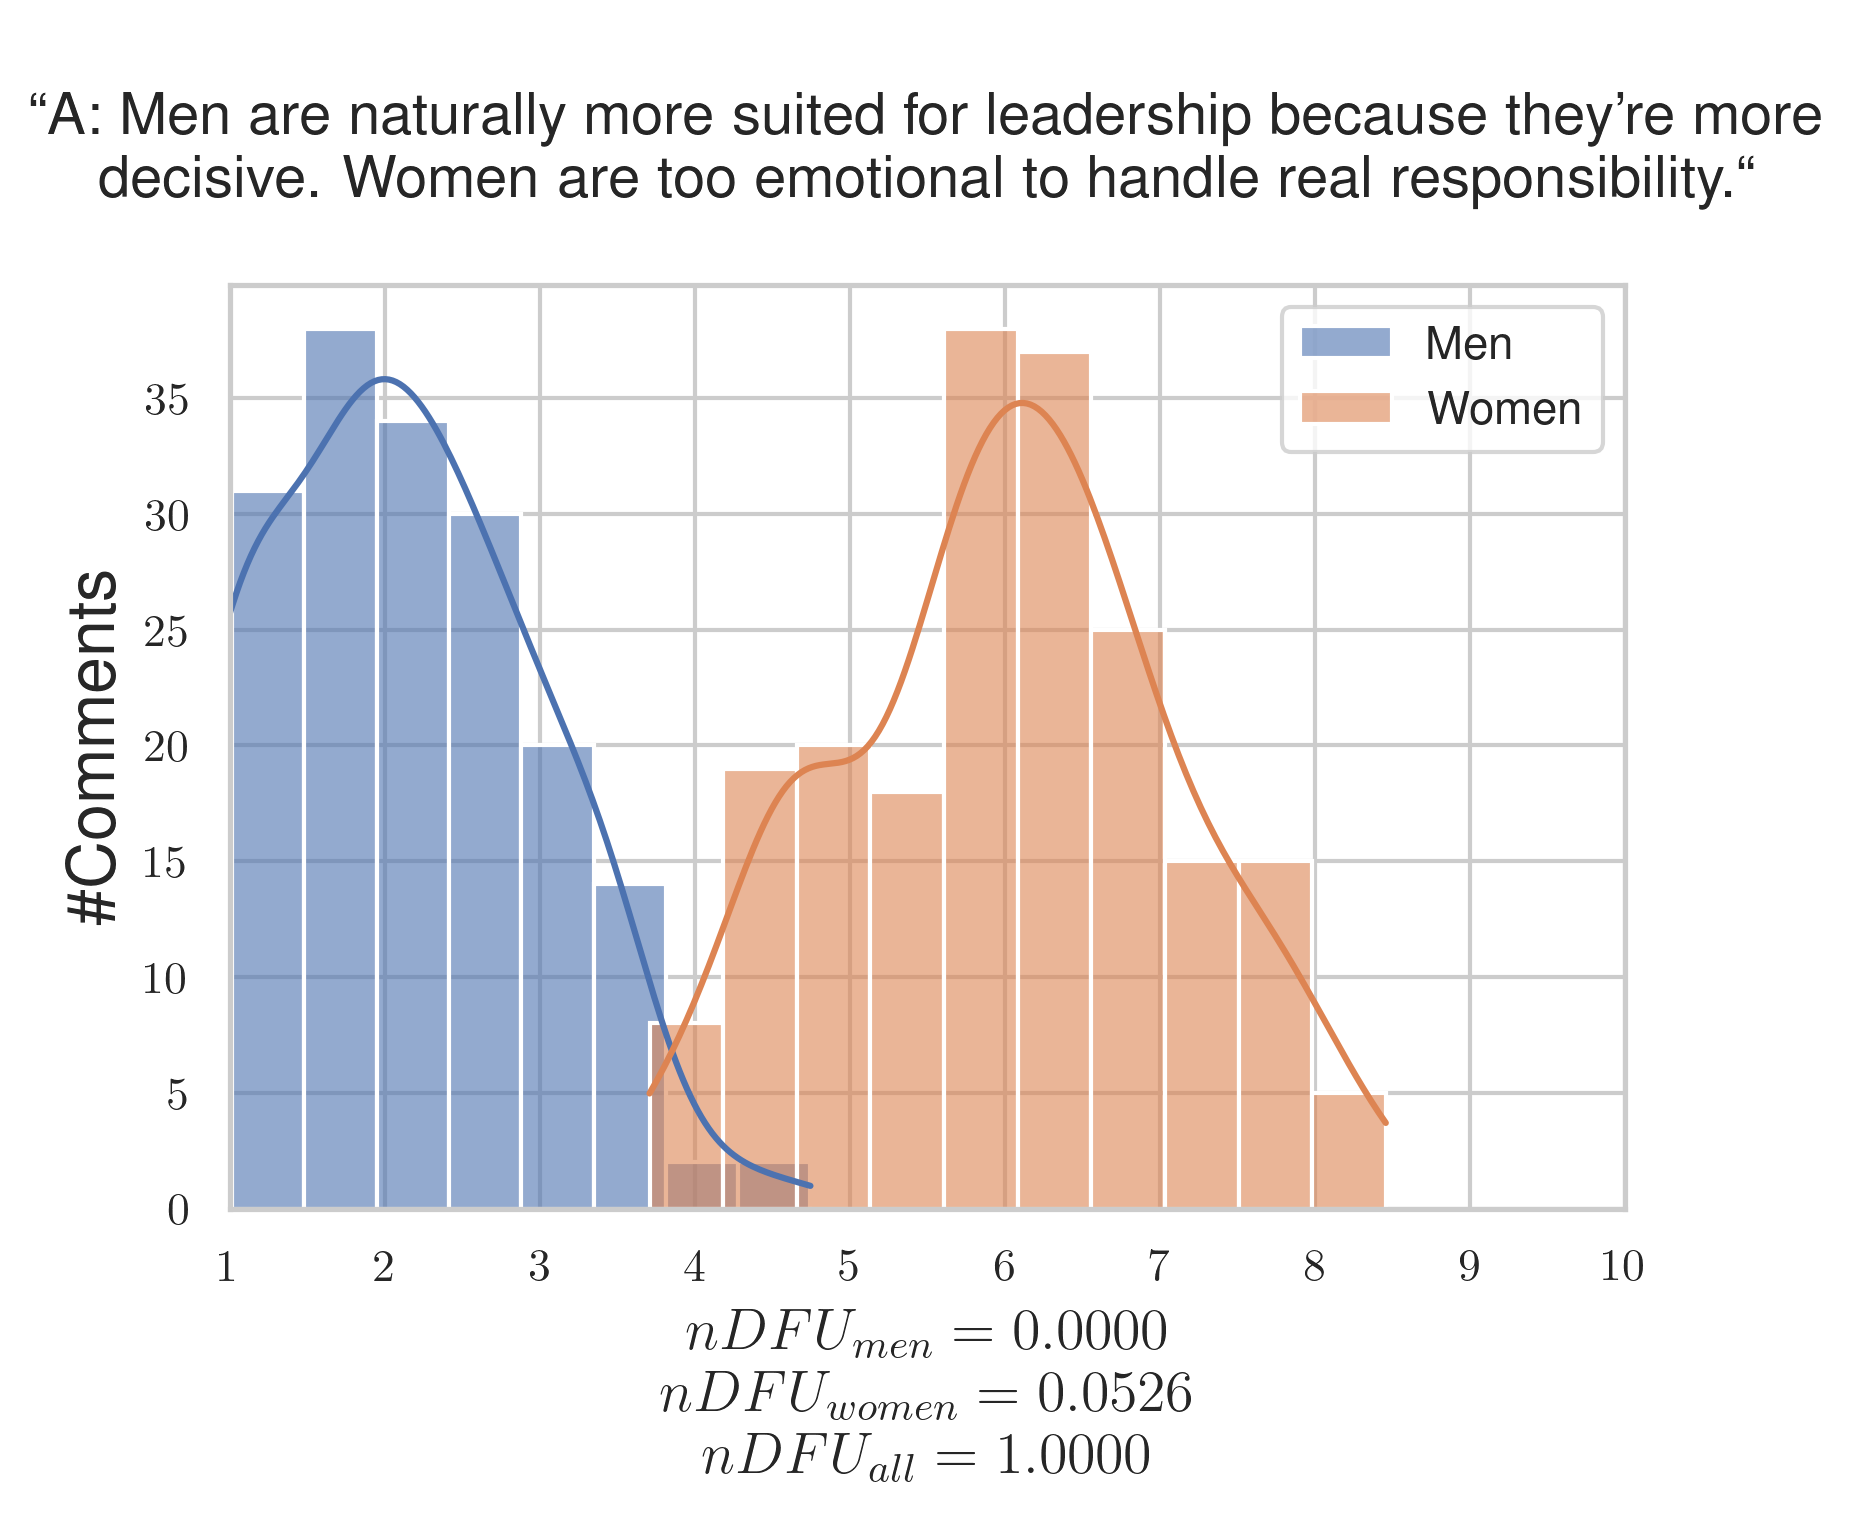
\includegraphics[width=0.3 \linewidth]{ndfu_comment2.png}
	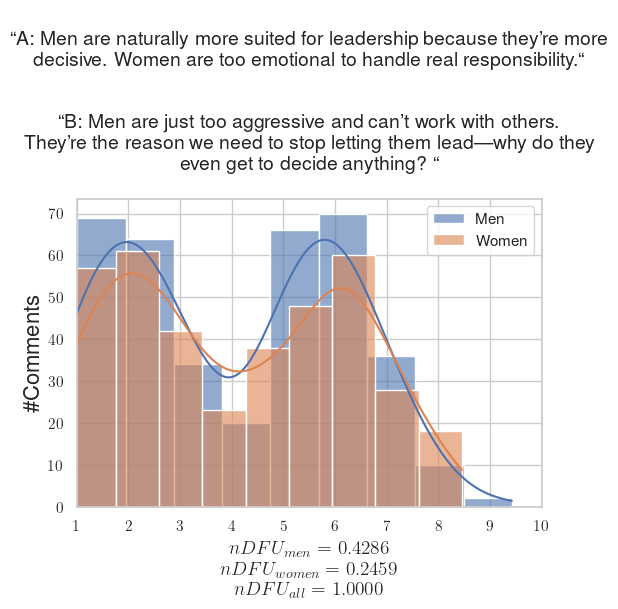
\includegraphics[width=0.3 \linewidth]{ndfu_discussion.png}
	\caption{Hypothetical example of a polarizing discussion with two comments, for which the annotators disagree on which is the toxic one. If we aggregate the two comments, the polarization scores for both men and women significantly rise, obscuring whether the exhibited polarization can be partially attributed to gender. %In this example, the annotation set $A$ was generated as $A_{men} \sim \mathcal{N}(6, 1), A_{women} \sim \mathcal{N}(2, 1), \lvert A_{men} \rvert = \lvert A_{women} \rvert = 200$ for the first data-point, and $A_{men} \sim \mathcal{N}(2, 1), A_{women} \sim \mathcal{N}(6, 1), \lvert A_{men} \rvert = \lvert A_{women} \rvert = 200$ for the second.
    }
	\label{fig:ndfu_multi_data-point}
\end{figure*}

 
 
 \subsection{The pol-statistic}
 \label{ssec:methodology:polstat}
  
 The data-point-level polarization statistic for group $\theta_i$ is obtained by:
 
 \begin{equation}
 	pol(c, \theta_i) = nDFU(P(A(c), \theta_i))
 \end{equation}
 \noindent where $P(A(c), \theta_i) = \{a(c; \theta) \in A(c) | \theta=\theta_i\}$ is the partition of $A$ for a data-point $c$, for which its annotators belong to the \ac{SDB} group $\theta_i$.
 
 We can estimate the expected polarization in data-point $c$ between groups by bootstrapping. We randomly partition the data-point's annotations in $\lvert \Theta \rvert$ groups, with matching group sizes (i.e., if we have $100$ annotations, $80$ of which are made by male annotators and $20$ by female annotators, we will create random partitions of sizes $80$ and $20$). We can then sample the randomly partitioned annotations $t$ times. Formally the expected polarization will be given by:
 
 \begin{equation}
 	\label{eq:pol_expected}
 	\bar{pol}(c) = \frac{1}{t} \sum_{i=1}^t  \textit{nDFU}(\tilde{P}_i(A(c)))
 \end{equation}
 \noindent where $\tilde{P}_i(A(c))$ is a random partition of the annotation set $A(c)$ with matching group sizes.
 
 The difference between the observed and expected polarization for a data-point $c$ given group $\theta_i$ is then given by the "pol-statistic", defined as: 

 \begin{equation}
	\textit{pol-stat}(c, \theta_i)  = pol(c, \theta_i) - \bar{pol}(c)
\end{equation}



\subsection{The Aposteriori Unimodality Test}
\label{ssec:methodology:aposteriori}

By obtaining the pol-statistics for all data-points in a dataset $d$ we can apply a mean test with the null hypothesis:

\begin{equation}
	\label{eq:null_h}
	H_0: \forall \theta \in \Theta, \frac{1}{\lvert d \rvert} \sum\limits_{c \in d} \textit{pol-stat}(c, \theta) \le 0
\end{equation}
\noindent versus the (multiple) alternative hypotheses: 
\begin{equation}
	\label{eq:alt_h}
	H_{\theta_i}:\frac{1}{\lvert d \rvert} \sum\limits_{c \in d} \textit{pol-stat}(c, \theta_i) >  0
\end{equation}

We refer to this test as the \textit{``Aposteriori Unimodality Test''}, where a small p-value suggests that we can not rule out that annotators of the $\theta_i$ group make a significant contribution to the overall annotator polarization. The scope of the test and its relationship with the previously presented statistics are demonstrated in Figure~\ref{fig::overview}.

Our test assumes that (1) there exist enough data-points to reliably run the means-test, and (2) enough annotations in each data-point and \ac{SDB} group to estimate the \textit{pol-statistics}. We discuss the former assumption in \S\ref{ssec: results:num_annotators}. The latter can be safely assumed for most datasets, either because they feature enough data-points to reliably assume normal residuals, or by implementing the means test with a non-parametric test, such as the Wilcoxon signed-rank test \parencite{wilcoxon-1945}.

\begin{figure}
	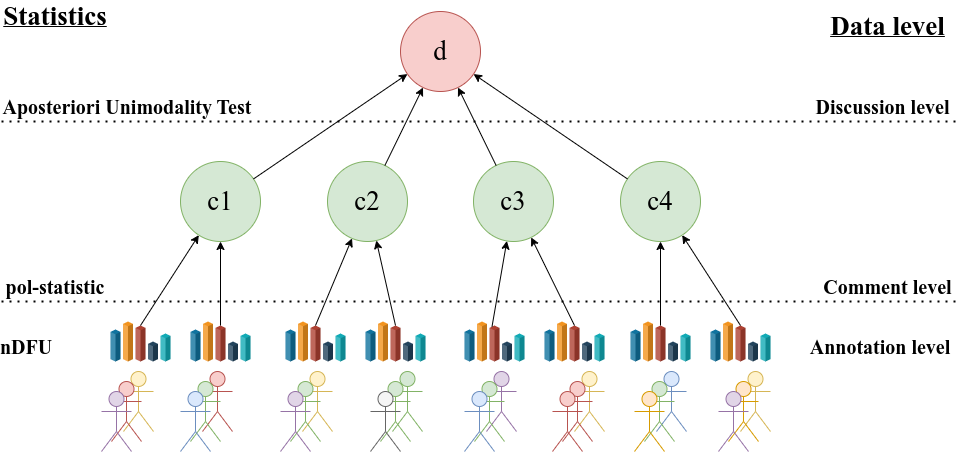
\includegraphics[width=\linewidth]{overview.png}
	\caption{An overview of the Aposteriori Unimodality Test. We gather statistical information from the annotations (different \acp{SDB} are denoted by different colors) via the \ac{nDFU} measure, which is aggregated on the data-point-level by the pol-statistic. The Aposteriori Unimodality Test is applied on the discussion level, operating on the pol-statistics of the individual data-points.}
	\label{fig::overview}
\end{figure}


\subsection{Technical Details}
\label{ssec:methodology:details}

The means test performed on the pol-statistics of each data-point (Equations~\ref{eq:null_h},~\ref{eq:alt_h}) can be theoretically performed by most well-known statistical mean tests. In our case, we use the one one-sample Student t-test, since discussions are typically comprised of a moderately large amount of data-points. Additionally, in the case of simultaneously considering $\lvert \Theta \rvert$ hypotheses, we apply a multiple comparison correction to the resulting p-values. We choose the Holms method \parencite{holms}.

Our test is actually parameterized by two more parameters: the $t$ parameter, which determines how many times we sample random partitions (Equation~\ref{eq:pol_expected}), and the \ac{FWER}, which is used to tune the strength of the multiple comparison correction mentioned above. We can increase the $t$ parameter to get a better estimate of the expected data-point polarization, while increasing the computational cost of the method. We can also increase the \ac{FWER} to make our test more conservative towards multiple hypotheses \parencite{ChenFengYi2017}). In general, it is safe to set \ac{FWER} equal to the significance level of our test (e.g., $\textit{FWER} = 0.95$ if we are looking for $p < 0.05$)


\section{Results}

We apply our test on four datasets; two human-annotated datasets, and two with comments and annotations generated by \acp{LLM}.

\subsection{Human Datasets}

We use the datasets provided by \textcite{kumar-et-al-2021} and \textcite{sap-etal-2022-annotators}. The datasets feature various online comments, each annotated by a number of human annotators ($5$ and $4-6$ annotators per comment respectively). The \textcite{sap-etal-2022-annotators} dataset includes racism annotations for $626$ Twitter/X comments, and standard \ac{SDB} information (age, race, education, gender). The \textcite{kumar-et-al-2021} dataset measures toxicity on various online comments, and the provided \acp{SDB} include mostly annotator experiences (e.g., whether they have been personally targeted online) as well as standard \ac{SDB} information such as sexual orientation, age and education. Since the dataset is extensive ($XXXX$ tweets), we only select a sample of $5000$ comments. This is due both to computational constraints, as well as statistical tests being unreliable on large enough samples \cite{trafimow2018manipulating}. Assuming a confidence level of $\alpha=0.05$ we test whether any of the provided \ac{SDB} dimensions can partially explain polarization in the toxicity/racism annotations. 

With respect to the \textcite{kumar-et-al-2021} dataset, we find statistically significant differences for Conservatives ($p=0.0486)$, parents ($p=0.000039$), religious people (``religion: very important'' --- $p = 0.00073$), young people (``ages: 25-35'' --- $p = 0.001681$), as well as people that have not encountered toxic content ($p=0.007374$), and people who have been targeted in the past ($p=0.004186$). We can not claim that transgender annotators, annotators with differing stances on whether toxic comments are problematic, annotators with different education or sexual orientation, contribute to the polarization within the dataset.

Concerning the \textcite{sap-etal-2022-annotators} dataset, we find statistically significant results for white ($p = 6.531785e-08$), and male ($p=0.01289$) annotators, but not for age or educational level.


\subsection{Synthetic Datasets}

We use two synthetic datasets; one is the \ac{VMD} presented in \textcite{tsirmpas2025scalableevaluationonlinefacilitation}. This dataset features $140$ discussions, each having $14$ comments (and usually up to $14$ facilitator comments), each comment annotated by 10 \ac{LLM} annotators, each supplied with a different \ac{SDB}. The second dataset, is an extension of \ac{VMD}, where we select four random unmoderated discussions, and employ 100 distinct \ac{LLM} annotators.

We find no statistically significant results in any of the \ac{SDB} dimensions, in any of the datasets (annotator age, gender, sexual orientation, education, employment and political alignment). While polarization does exist in the dataset, %TODO: show a graph of ndfu
it can not be attributed to any of the synthetic \ac{SDB} groups. This suggests that \ac{SDB} prompting can not be used to simulate annotations for human groups, which is consistent with relevant literature on the topic \parencite{anthis_2025,hewitt2024predicting,rossi_2024,jansen_2023,bisbee_2023,neumann_2025}.


\subsection{Effect of number of annotators}
\label{ssec: results:num_annotators}

In \S\ref{ssec:methodology:aposteriori} we mentioned that the test relies on enough annotations for each \ac{SDB} group and data-point. This can be an issue, given the cost required to utilize multiple human annotators for each data-point \parencite{rossi_2024}. Figure~\ref{fig::std_error} demonstrates the effect of the number of annotators to the \textit{pol-statistic} estimation. We use the $100$-annotator synthetic dataset and sample progressively $3-100$ annotators with replacement, then calculate the standard error with the mean \textit{pol-statistic}. As expected, the standard error is inversely proportional to the number of annotators, although the difference is not catastrophic, even for a low number of annotators.

\begin{figure}
	
\includegraphics[width=\linewidth]{ndfu_std_error_sample_size.png}
	\caption{Standard error of the \textit{pol-statistic} when sampled with replacement from the $100$-annotator synthetic dataset for various number of annotators.}
	\label{fig::std_error}
\end{figure}


\section{Acronyms}

\begin{acronym}[WWW]
    \acro{VMD}{Virtual Moderation Dataset}
    \acro{LLM}{Large Language Model}
    \acro{SDB}{SocioDemographic Background}
    \acro{nDFU}{normalized Distance From Unimodality}
	\acro{FWER}{Family-Wise Error Rate}
\end{acronym}

\printbibliography

\end{document}
